\documentclass[11pt]{article}
\usepackage{amsmath,amsfonts,bm,wrapfig}
\usepackage[left=1in,right=1in,top=1in,nohead]{geometry}
\usepackage[dvips]{graphicx}
\usepackage[
pdftitle={nsf si2 bie},
pdfcreator={pdftex}, 
pdfsubject={paper},
pdfkeywords={some,topics},
hyperindex = {true},  % turn to false for final
colorlinks = {true},  % turn to false for final
linkcolor = {blue},
pagecolor = {blue},
citecolor = {blue}
]{hyperref}
\usepackage{nsf}
\usepackage{paralist}
\usepackage{todonotes}
\usepackage{stmaryrd}
\usepackage{tikz,pgfplots}

\usepackage[T1]{fontenc}
\usepackage{ae,aecompl}
\usepackage[labelfont=it,,textfont=it,font=footnotesize]{caption}
\captionsetup{belowskip=-20pt}
%
%\newcommand{\subfigimg}[3][,]{%
%  \setbox1=\hbox{\includegraphics[#1]{#3}}% Store image in box
%  \leavevmode\rlap{\usebox1}% Print image
%  \rlap{\hspace*{-10pt}\raisebox{\dimexpr\ht1-0\baselineskip}{
%  \scriptsize #2}}% Print label
%  \phantom{\usebox1}% Insert appropriate spacing
%}


%%\topmargin=-13.5mm
%\topmargin=-14.0mm
%%\topmargin=7mm
%%\textheight=22.8cm
%\textheight=23.0cm
%%\textheight=23.3cm


%\parindent=0mm
%\parskip=2mm

%%\textwidth=16.1cm
%\textwidth=16.5cm
%\evensidemargin = -1mm
%\oddsidemargin = -1mm

%\renewcommand{\baselinestretch}{1.05}

\usepackage{amssymb}
\usepackage{epsf,color}

\input vs_macros.tex

%\newcounter{sectnumber}
%\newcounter{subsectnumber}[sectnumber]


%\renewcommand{\section}[1]{
%\stepcounter{sectnumber}
%{\large\bf \arabic{sectnumber}. #1}
%}

%\renewcommand{\subsection}[1]{
%\stepcounter{subsectnumber}
%{\bf \arabic{sectnumber}.\arabic{subsectnumber}. #1}
%}
%
%\usepgfplotslibrary{external}
%\tikzexternalize


\begin{document}


\noindent
\begin{center}
{\large \bf 
%Mechanobiology of the Primary Cilium and Its Role in 
%Cellular Cycles of Mechanosensing, Mechanotransduction and Mechanoresponse
%MPS-BIO: Collaborative Research: Mathematical Modeling of Mechano-chemistry of Primary Cilium\\}
%Collaborative Research: 
Collaborative Research: Osmophoresis: propulsion of semipermeable vesicles driven by chemical gradients\\}
{\it Sangwoo Shin (University of Hawaii at Manoa) and Yuan-Nan Young (NJIT)}
\end{center}

%%%%%%%%%%%%%%%%%%%%%%%%%%%%%%%%%%%%%%%%%%%%%%%%%%%%%%%%%%%%%%%%%%%%%%%%
\section{Introduction: Osmophoresis as a biological jet engine}

This collaborative proposal aims to (1) characterize osmophoresis
quantitatively by both microfluidic experiments, theoretical modeling,
and numerical simulations, and (2) explore applications of osmophoresis
in biological fluid dynamics.  Osmosis is the motion of fluid generated
by a solute concentration gradient across a semipermeable membrane
(e.g., lipid bilayer membrane) that allows only small molecules (such as
solvent) to transport across the membrane, but not large solute
molecules~\cite{anderson1974}.  When a vesicle, an object enclosed by
semi-permeable membrane, is exposed to a local solute concentration
gradient, the net osmotic solvent flow across the semi-permeable
membrane results in the motion of the vesicle, a process referred to as
{\em osmophoresis}~\cite{anderson1983,anderson1986,gordon1981}.  The
contrast in solute concentration across the vesicle induces a net
solvent flow that pushes the vesicle to move from high to low solute
concentration. Such osmophoretic motion is against the gradient in
osmotic pressure, which is proportional to the solute concentration.

Osmosis is common in biology as cells and microorganisms with a large
range of water permeabilities in their membranes~\cite{deamer1986,
finkelstein1976, lawaczeck1979} are immersed in solutions containing
impermeable solutes which are typically distributed non-homogeneously,
implying osmophoresis could also be a common phenomenon in nature.
Figure~\ref{fig:illustration}a summarizes the physical mechanism behind
osmophoresis, where the propulsion of a vesicle via osmophoresis is
driven by a fluid flow {\em through} its body in the opposite direction,
which is analogous to how a jet engine acquires its thrust by propelling
the air backwards (Figure~\ref{fig:illustration}b). 
\begin{figure}[h]
\begin{center}
\includegraphics*[keepaspectratio=true,width=\textwidth]{figs/Illustration_Osmosis.pdf}
\caption{Osmophoresis: a biological jet engine powered by chemical
  gradients. (a) A semi-permeable vesicle can uptake fluid from the
  front and expel fluid to the rear due to osmotic pressure imbalance
  induced by the solute concentration gradient, thus producing thrust,
  (b) which is analogous to a jet engine.}
\label{fig:illustration}
\end{center}
\end{figure}

Although the basic physical mechanism of osmophoresis is comprehensible,
past work on osmophoresis (both theoretical and experimental) failed to
provide a complete explanation for contradicting findings of the
dependence of osmophoretic velocity on various factors such as fluid
viscosity and vesicle radius~\cite{anderson1983, anderson1986,
gordon1981, nardi1999}. \todo[inline]{Must be other unknowns such as
distribution of semi-permeable regions}  One reason for the lack of
detailed investigation on osmophoresis is attributed to the fact that
the osmophoresis is a completely different propulsion mechanism from
other common phoretic swimming strategies such as diffusiophoresis,
electrophoresis, and thermophoresis. Such a phoretic swimming is driven
by an interfacial fluid flow that occurs along the particle surface due
to the interaction between the particle and the fluid whereas {\bf
osmophoresis is driven by the fluid flow through the particle interior
due to osmosis}, which does not require any surface
interactions~\cite{anderson1986,anderson1989}. The PIs hypothesize that
such a mechanism, which is largely under-appreciated by the community,
is actually more likely to occur in nature than other phoretic motions
due to the abundance of the chemical gradients in biological
environments. \todo[inline]{Reviewer 1 is critical that there is not
enough evidence that osmophoresis is likely to be more important than
the other methods of transport} Recent reports on the dynamics of {\em
E.~Coli}~\cite{rosko2017} and tumor cells~\cite{stroka2014} induced by
osmotic pressure gradients also strengthen this speculation. 

Based on the preliminary results in~\S\ref{sec:preliminary_results}, the
PIs propose to investigate the dependence of osmophoresis on various
physical parameters such as the vesicle size, fluid viscosity, and
mechano-chemical processes.  Results from the proposed experiments will
enable the PIs to validate the mathematical model and numerical
simulations.  These results will allow PI Shin to synthesize a vesicle
to closely mimic the actual cellular environment and address how
osmophoresis can impact the dynamics of various biological events such
as polarized cellular growth and bacterial locomotion.  The PIs will
also address the potential applications of osmophoresis for various
systems such as biological self-organization and targeted drug delivery.

Figure~\ref{fig:synergy} highlights the synergy between experiments
(Sangwoo Shin, SS), modeling (Yuan-Nan Young, YNY), and numerical
simulations (Bryan Quaife, BQ): The {\bf objective} of this project is
to conduct experimental characterization, theoretical modeling, and
numerical simulations of osmophoresis, leading to a deeper and
quantitative understanding to address the unresolved issues.  Once
constructed a theoretical model validated by experiments, the PIs will
investigate osmophoresis in realistic cellular environments to quantify
the role of osmophoresis in the dynamics of micro-organisms.  Finally
the PIs will investigate the efficiency of osmophoresis for
biological/biomedical applications such as guided self-assembly via
chemical gradients and targeted drug delivery in confined spaces.
%
\begin{figure}[h]
\begin{center}
\includegraphics*[keepaspectratio=true,scale=0.375]{figs/Synergy.pdf}
\caption{\label{fig:synergy} Synergy between experiment and modeling:
  Experimental characterization of osmophoresis will be synergized by
  theoretical modeling, leading to deeper and quantitative understanding
  of the phenomenon. Together the PIs will  further  investigate
  osmophoresis in biological environment as well as address osmophoresis
  in possible applications. See~\S\ref{sec:ProposedResearch} for more
  details.}
  \todo[inline]{update the figures to include numerical methods}
\end{center}
\end{figure}
%%  	

\noindent
{\bf Intellectual Merit:}
The proposed investigation will include experimental studies of the
vesicle motion via osmophoresis under various parameters such as vesicle
type and size, where we use microfluidic methods to control the
properties and experimental conditions, and optical microscopy combined
with image analysis to quantify the motion of the vesicles. We will also
utilize numerical simulations and reduced-order analytical models to
gain further insights into the experimental observations.
\todo[inline]{Reviewer 2 wanted to see more on reduced order models and
numerics in general}

This collaborative proposal will investigate osmophoresis as an
effective propulsion mechanism for semi-permeable vesicles.  Largely
overlooked by the engineering community because of the apparent
similarities to other phoretic mechanisms, there is a lack of knowledge
in understanding osmophoresis.  In this regard, the experimental and
theoretical work investigating the dynamics of osmophoresis of
semipermeable vesicles will be a new addition to the library of known
propulsion mechanisms for colloidal biomaterials.  Moreover, since the
vast majority of the biological entities are bound by semipermeable
membranes, osmophoresis is expected to play a major role in biological
motility.  In addition to being a biological driving force, osmophoresis
can be an alternate driving mechanism for various systems such as
chemically-guided self-organization of vesicles that may shed light on
the formation of protocells, or delivering drugs cargos in deep,
confined pores such as tumors or intestine, which could offer more
effective way of achieving targeted drug delivery.

\noindent
{\bf Broader Impact:} 
The CBET Fluid Dynamics Program describes its mission as to support
fundamental research toward gaining an understanding of the physics of
various fluid dynamics phenomenon. The description also highlights one
of the main programs as Bio-inspired Fluid Mechanics, which includes
fluid-structure interactions and biological flow processes. The PIs
emphasize that the osmophoresis is indeed a consequence of a fluid
(solution)-structure (membrane) interaction that is likely to take place
in various biological systems.  Another important broader impact of this
proposal is the education and training of both undergraduate and
graduate students in mechanical engineering and applied math.  The
combination of microfluidic experiments, mathematical modeling and
numerical simulations in this project provide a compelling example of
the importance of theoretical modeling. The proposed experimental and
modeling approaches will lead to a better understanding of osmophoresis
and its roles in cellular dynamics and propulsion.  Development of
mathematical analysis, and numerical methods to understand these
processes will be of great benefit for understanding experimental
observations and improving technology.  The concepts and methods
described here go beyond the context of osmophoresis and extend to other
problems featuring mechanically induced cellular function.

%%%%%%%%%%%%%%%%%%%%%%%%%%%%%%%%%%%%%%%%%%%%%%%%%%%%%%%%%%%%%%%%%%%%%%%%
\section{Preliminary Results\label{sec:preliminary_results}} The PIs
have research capabilities to conduct both experiments (SS), modeling
(YNY), and numerical simulations (BQ) to investigate the motion of
colloidal particles via solute gradients.  Using the developed
experimental setup and numerical modeling, the PIs propose to
investigate osmophoresis as a propulsion mechanism for both vesicles and
biological cells. 

%%%%%%%%%%%%%%%%%%%%%%%%%%%%%%%%%%%%%%%%%%%%%%%%%%%%%%%%%%%%%%%%%%%%%%%%
\subsection{Experimental Tools (PI Sangwoo Shin)}
\label{subsection:exp_tools}
%%%%%%%%%%%%%%%%%%%%%%%%%%%%%%%%%%%%%%%%%%%%%%%%%%%%%%%%%%%%%%%%%%%%%%%%
The experimental research will be conducted at PI Shin's lab at the
University of Hawaii at Manoa.

%%%%%%%%%%%%%%%%%%%%%%%%%%%%%%%%%%%%%%%%%%%%%%%%%%%%%%%%%%%%%%%%%%%%%%%%
\subsubsection{Microfluidics for evaluating the motion of particles
driven by chemical gradients}
\label{subsubsec:microfluidics}
%%%%%%%%%%%%%%%%%%%%%%%%%%%%%%%%%%%%%%%%%%%%%%%%%%%%%%%%%%%%%%%%%%%%%%%%
PI Shin has demonstrated a microfluidic tool for quantifying colloidal
migration induced by solute gradients that can be easily compared to an
analytical solution for the transient solute concentration profile in a
finite space~\cite{shin2016,shin2017a,shin2017b}. The device is
comprised of a shallow dead-end pore connected to a large main channel
(Figure~\ref{fig:fig3}a).  To impose a solute gradient along the
dead-end pore, we have used a microfluidic approach, where the entrance
of the dead-end channel is connected to the main flow channel so that
the solute concentration ($c_o$) can be regulated at the entrance.
Additionally, the height of the dead-end channel is much thinner
($\approx 10 \mu$m) than the main channel ($\approx 100 \mu$m), such
that the advective disturbance from the main channel can be minimized.
%
\begin{figure}[h]
\begin{center}
\includegraphics*[keepaspectratio=true,scale=1]{figs/fig3.pdf}
\caption{\label{fig:fig3} A microfluidic platform for characterizing
  particle motion induced by solute gradients~\cite{shin2016,
  shin2017a}. (a) Setup for experiments in a dead-end channel adjacent
  to a main flow. (b) Step-like initial solute and colloid
  concentrations are realized by inserting an oil drop or air bubble
  between two liquids with different solute concentrations. (c)
  Otherwise, a gradual concentration gradient occurs due to mixing.
  Insets in (b) and (c) are the fluorescent intensity distributions of
  colloidal particles (polystyrene (PS) beads, diameter $0.19 \mu$m)
  along the channel. Scale bars are $50 \mu$m.}
\end{center}
\end{figure}
%%  	

Furthermore, unlike electro- or thermo-phoresis where the external field
gradient is typically constant, diffusion in a dead-end configuration is
time dependent, as occurs when a change in chemical concentration occurs
at the pore entrance. To observe the dynamics, experiments utilizing a
step-like initial concentration profile are desired since the solution
to diffusion equation in a finite space with a constant boundary
condition is readily available.  \todo[inline]{Reviewer 1 argued that a
gradual concentration gradient should be examined since this is what
would occur because of mixing} We designed such microfluidic experiments
(Figure~\ref{fig:fig3}b) by inserting in the main channel an
immiscible fluid, e.g.~an oil droplet or air bubble, to separate the
leading solution, which fills in the dead-end channel with concentration
$c_i$, with a second immiscible solution that has different solute
conditions (concentration $c_o$) and contains the colloidal particles
(Figure~\ref{fig:fig3}b). This sequential approach works as an effective
gate leading to a repeatable constant inlet concentration at the start
of the experiment. In the absence of this flow design, the trailing
fluid that contains the colloidal particles will be mixed with the
leading fluid during the delivery to the inlet of the dead-end channel.
This results in $> 10$ min of dead time before the steady-state inlet
condition is reached (Figure~\ref{fig:fig3}c); such a delay would
obscure and compromise the results we propose to investigate.

%%%%%%%%%%%%%%%%%%%%%%%%%%%%%%%%%%%%%%%%%%%%%%%%%%%%%%%%%%%%%%%%%%%%%%%%
\subsubsection{Flow-induced synthesis of giant unilamellar vesicles
(GUVs)}
\label{subsubsec:GUVs}
%%%%%%%%%%%%%%%%%%%%%%%%%%%%%%%%%%%%%%%%%%%%%%%%%%%%%%%%%%%%%%%%%%%%%%%%
In addition to the conventional electroformation for producing giant
unilamellar vesicles (GUVs), PI Shin has demonstrated a flow-based
method to synthesize GUVs with a uniform vesicle
diameter~\cite{shin2015}.  It is known that a fusion between suspended
lipid vesicles is difficult to achieve without mediators such as
membrane proteins or ions because the vesicles have extremely low
equilibrium membrane tension~\cite{jahnig1996} and high poration
energy~\cite{gao2008}.  Nonetheless, vesicle fusion in the absence of
mediators can also be achieved by mechanical forcing that is strong
enough to induce membrane poration such as fluid shear stress.  By
utilizing a unique vortex formation phenomenon in branched channels
(Figure~\ref{fig:fig4}a) as a platform for capturing, stressing, and
fusing the lipid vesicles, we have directly visualized using high-speed
imaging the vesicle fusion events, induced solely by shear, on the time
scale of submilliseconds (Figure~\ref{fig:fig4}b). A large vesicle with
a size of up to $\approx 10\mu$m can be achieved by the fusion of
nanoscale vesicles.  This study has also shown that the size of GUVs can
be controlled by simply changing the size of the channel dimensions.
This method allows a rapid formation of GUVs with various size with ease
whereas the electroformation method is time-consuming and requires
additional devices such as an external power supply and electrodes.
%
\begin{figure}[h]
\begin{center}
\includegraphics*[keepaspectratio=true,scale=1]{figs/fig4.pdf}
  \caption{\label{fig:fig4} Formation of GUVs via vortex trapping in
  branching channels~\cite{shin2015}. (a) Numerical simulation of the
  flow streamlines within the channel, revealing vortex breakdown near
  flow junctions.  (b) High-speed imaging of a GUV produced by merging
  of small vesicles (SUVs) that are trapped inside the vortex.}
\end{center}
\end{figure}
%%  	

%%%%%%%%%%%%%%%%%%%%%%%%%%%%%%%%%%%%%%%%%%%%%%%%%%%%%%%%%%%%%%%%%%%%%%%%
\subsubsection{Motion of lipid vesicles in dead-end pores under osmotic
pressure gradient}
\label{subsubsec:osmophoresis_lipid_vesicles_deadend_pores}
%%%%%%%%%%%%%%%%%%%%%%%%%%%%%%%%%%%%%%%%%%%%%%%%%%%%%%%%%%%%%%%%%%%%%%%%
As a proof of concept, we have conducted preliminary experiments on
osmophoresis using the dead-end method developed by PI
Shin~(\S\ref{subsubsec:microfluidics}).  The GUVs were made via standard
electroformation method, which has an average diameter of around $1
\mu$m. The GUVs consist of DOPC
(1,2-dioleoyl-sn-glycero-3-phosphocholine) and DPPE
(1,2-dipalmitoyl-sn-glycero-3-phosphoethanolamine).  By establishing a
concentration gradient of sucrose along the dead-end pores, we have
observed a significant motion of GUVs directing toward the pore end with
average speed of $\mathcal{O}(10 \mu$m/s), (see Figure~\ref{fig:fig5}).
Otherwise, in the absence of sucrose gradients, no vesicle motion into
the pore is observed.
%
\begin{figure}[h]
\begin{center}
\includegraphics*[width=\textwidth]{figs/fig5.pdf}
\caption{\label{fig:fig5} Motion of phospholipid GUVs driven by solute
  gradient. The dead-end pores initially contain 0.1 mM of sucrose
  solution while the solution in the main channel contains 100 mM
  sucrose solution with GUVs.  The solute gradient is established as
  soon as the main flow passes over the dead-end pores.}
\end{center}
\end{figure}
%%  	
Since sucrose is a non-electrolytic solute, electrolytic
diffusiophoresis can be neglected in this case.  And non-electrolytic
diffusiophoresis can be neglected since it directs particles toward
higher concentration region and it is also significantly small compared
to electrolytic diffusiophoresis.  These preliminary results suggest
that osmophoresis is the key mechanism that is responsible for such a
directed vesicle motion as the vesicles are shown to move down the
solute gradient even with non-electrolytic solutes.  Therefore, we
believe we have shown the potential of osmophoresis to be a strong
propulsion mechanism for any objects that are enclosed by a
semipermeable membrane including vesicles (liposomes), cells, and
bacteria.

%%%%%%%%%%%%%%%%%%%%%%%%%%%%%%%%%%%%%%%%%%%%%%%%%%%%%%%%%%%%%%%%%%%%%%%%
\subsection{Mathematical modeling of a soft porous drop in Stokes flow} 
\label{subsec:math_modeling}
%%%%%%%%%%%%%%%%%%%%%%%%%%%%%%%%%%%%%%%%%%%%%%%%%%%%%%%%%%%%%%%%%%%%%%%%
PI Young has modeled and simulated vesicle
hydrodynamics~\cite{Veerapaneni2011_PRL, Vlahovska2011_JFM} and
electrohydrodynamics~\cite{HuLai2016_JCP, Nganguia2013_PRE}.  In
addition, PI Young also investigated how the tension in the membrane may
deform a transmembrane protein as a vesicle deforms in response to shear
stress in microfluidic devices~\cite{Pak2015_PNAS, Peng2016_AMS}. Inside
a cell, the enclosed fluid is a suspension (of macromolecules such as
proteins and enzymes, ions, and filaments) often modeled as a soft
porous structure immersed in a viscous fluid.  Such intracellular soft
porous medium can be modeled as a two-phase fluid system, with a fluid
phase (subscript $``f"$) and a soft solid structure phase (subscript
$``s"$).  The governing equations for the two-phase system
are~\cite{Young2019_PRF}
\todo[inline]{Yuan: This is your paper with Miksis and Mori. Is this the
correct one?}
\begin{align}
\label{eq:geq1}
\frac{\partial \phi_f}{\partial t} + \nabla \cdot \left({\bf v}_f \phi_f\right) &= 0,\;\; \nabla \cdot \left(\phi_f {\bf v}_f + \phi_s {\bf v}_s \right) =0,\;\;\phi_f + \phi_s = 1,\\
%
\label{eq:geq2}
\nabla \cdot {\tau}_f -\phi_f \nabla p +\xi\left({\bf v}_f - {\bf v}_s\right) &=0,\;\; \tau_f\equiv \frac{\nu_i}{2}\left(\nabla {\bf v}_f + \left(\nabla{\bf v}_f\right)^T\right), \\
%
\label{eq:geq3}
\nabla \cdot {\tau}_s-\phi_s \nabla p -\xi \left({\bf v}_s - {\bf v}_f\right) &=0,\;\; \tau_s\equiv \tau_{sv}+\tau_{se},
\end{align}
with $\phi_f$ $({\bf v}_f)$ the volume fraction (velocity) of fluid,
$\phi_s$  $({\bf v}_s)$ the volume fraction (velocity) of the porous
solid, $p$ the fluid pressure, $\nu_i$ the viscosity of interior fluid,
$\xi$ the drag coefficient between the skeleton and the viscous fluid,
$\tau_f$  the stress tensor in the interior fluid, and $\tau_s$ the
stress tensor in the skeleton. $\tau_s$ may consist of both a viscous
dissipation $(\tau_{sv})$ that depends on the rate of strain of the
porous solid and an elastic component $(\tau_{se})$ that depends on the
strain of the skeleton.  Often the elastic component dominates the
viscous component in $\tau_s$,  and in the small-strain limit the stress
in the skeleton can be approximated as
\begin{align}
\tau_s &\approx \tau_{se} = \bf{\Lambda}\mbox{tr}(\bf{\varepsilon}) \bf{I} + ({\cal M}-\Lambda) \bf{\varepsilon},\;\; 
{\bf \varepsilon} = \frac{1}{2}\left[\nabla {\bf u}_s + \left(\nabla {\bf u}_s\right)^T\right],
\end{align}
%
\begin{wrapfigure}[16]{l}{3.75in}
\centerline{\includegraphics[width=3.75in]{figs/DarcyDropUFlow0927aa.pdf}}
\smallskip\par
\centerline{\includegraphics[width=3.75in]{figs/BrinkmanDropUFlow0927aa.pdf}}
\vspace{-7pt}
\caption{\label{fig:DarcyDropUFlow0927} Streamlines around a soft Darcy
  (top panels) and Brinkman (bottom panels) drop in a uniform streaming
  flow.}
\end{wrapfigure}
%
with ${\bf u}_s$ the strain (displacement) of the skeleton, ${\bf
\Lambda}$ the Lam\'e's first parameter that depends on both bulk modulus
and shear modulus of the solid structure, $\mbox{tr}(\varepsilon)$ is
the trace of the strain tensor, and ${\cal M}$ is the p-wave modulus.
Equations~\eqref{eq:geq2} are the Brinkman equations when the fluid
viscous stress is comparable to the pressure gradient and the drag
force.  When the fluid viscous dissipation in equation (\ref{eq:geq2})
is neglected (often done in solid mechanics) the resultant equations are
Darcy's equations with a deformable underlying
skeleton~\cite{MacMinn2016_PRApplied}. Equations
\eqref{eq:geq1}--\eqref{eq:geq3} are the physically consistent
description of a soft porous drop with a deformable skeleton immersed in
a viscous fluid with a deformable fluid interface because the
displacement of the fluid interface has to be considered consistently
with the strain of the skeleton near the interface. Consistent boundary
conditions for the velocity at the boundary between the Stokes flow and
the porous flow are adopted from refs.~\cite{Angot2017_PRE,
MacMinn2016_PRApplied}.

The top row of Figure~\ref{fig:DarcyDropUFlow0927} illustrates the flow
around a soft Darcy drop in a uniform streaming flow (from left to
right), obtained by solving equations~\eqref{eq:geq1}--\eqref{eq:geq3}
with axial symmetry in the small-strain limit. When the Darcy drop is
not permeable, the streamlines go around the drop as in the case of a
viscous drop~\cite{DavisStone1993_CES,
GLeal_AdvancedTransportPhenomena}. At an intermediate permeability, flow
can penetrate through the soft Darcy drop, and the streamlines are
calculated to be parallel to the streaming direction ($z$-axis in this
case). At high permeability the streamlines go through the drop as if
there is no resistance from the skeleton to the streaming flow.  The
bottom row of Figure~\ref{fig:DarcyDropUFlow0927} summarize the flow
around a soft Brinkman drop in a uniform streaming flow with increasing
permeability.  We note that in the limit of zero permeability, the flow
around a Brinkman drop is almost identical to that around a Darcy drop.
At intermediate permeability the flow around a soft Brinkman drop
contains a saddle point that is often observed in non-Newtonian fluid
under shear.  As permeability increases the flow goes straight though
the drop as in the Darcy drop case.

%%%%%%%%%%%%%%%%%%%%%%%%%%%%%%%%%%%%%%%%%%%%%%%%%%%%%%%%%%%%%%%%%%%%%%%%
\subsection{High-fidelity numerical simulations of suspensions} 
\label{subsec:numerics}
%%%%%%%%%%%%%%%%%%%%%%%%%%%%%%%%%%%%%%%%%%%%%%%%%%%%%%%%%%%%%%%%%%%%%%%%
Vesicle suspensions in a Stokesian fluid can be reformulated as an
integral equation formulation~\cite{qua-bir2014, qua-bir2016}. A no-slip
boundary condition imposed on the $i^{\mathrm{th}}$ vesicle is 
\begin{align}
  \frac{d\xx_i}{dt} = \sum_{j=1}^{m} \SS_{ij}[\ff_j](\xx), \quad \xx
  \in \gamma_i,
  \label{eqn:bieTime}
\end{align}
where $S_{ij}$ is the Stokes single-layer potential and $\ff_j$ is the
membrane forces on the $j^{\mathrm{th}}$ body. Classically, the membrane
force includes a bending and tension force, but other forces, such as
adhesion~\cite{qua-vee-you2019}, can be included.

High-fidelity discretizations of equation~\eqref{eqn:bieTime} must address
nearly-singular integrands, numerical stiffness, multiple time scales,
and high-order derivatives. By using a near-singular integration scheme,
adaptive high-order time stepping, and Fourier differentiation, these
challenges have been addressed by PI Quaife~\cite{qua-bir2014,
qua-bir2016}. Figure~\ref{fig:stenosis} a stable simulation of a vesicle
passing through a constricted geometry.

\begin{wrapfigure}[]{l}{0.3\textwidth}
  \centering
  \includegraphics{figs/stenosisSnapsTime1.pdf}
  \includegraphics{figs/stenosisSnapsTime2.pdf}
  \includegraphics{figs/stenosisSnapsTime3.pdf}
  \includegraphics{figs/stenosisSnapsTime4.pdf}
  \caption{{fig:stenosis}Snapshots of a single vesicle in a constricted
  tube.  The boundary condition on the solid wall (plotted in blue) at
  the inlet and outlet is Gaussian-shaped, and on the remainder of the
  solid wall is zero.  The vesicle is initially $2.3$ times larger than
  the size of the constriction.}
\end{wrapfigure}


%%%%%%%%%%%%%%%%%%%%%%%%%%%%%%%%%%%%%%%%%%%%%%%%%%%%%%%%%%%%%%%%%%%%%%%%
\section{Summary}
\label{sec:summary}
%%%%%%%%%%%%%%%%%%%%%%%%%%%%%%%%%%%%%%%%%%%%%%%%%%%%%%%%%%%%%%%%%%%%%%%%
Osmophoresis, the propulsion of a semi-permeable vesicle driven by the
osmosis through the membrane, is hypothesized to be responsible for the
biological fluid dynamics that involve vesicle migration and assembly,
which are essential to many biological processes.  Due to the subtle
distinction between osmophoresis and other phoretic mechanisms,
osmophoresis remains relatively poorly quantified in terms of its roles
in biological fluid dynamics. 

In this proposal the PIs will first investigate osmophoresis as a
mechanical process and quantify the osmophoretic flow with experiments,
modeling, and numerical simulations.  Results from these proposed
research in \S\ref{subsec:aim1} will provide a quantitative description
of osmophoresis.  PI Shin has state-of-the-art experimental tools to
quantify osmophoresis of a phospholipid vesicle in various microfluidic
configurations.  In particular, the microfluidic configurations
discussed in \S\ref{subsubsec:osmophoresis_lipid_vesicles_deadend_pores}
are motivated by biological processes that involve vesicle transport
(see \S\ref{subsubsec:delivery_drug_cargos}).  PI Young has investigated
the hydrodynamics and electrohydrodynamnics of vesicles by both
asymptotic analyses and numerical simulations. Recently PI Young has
incorporated the porous medium (either Darcy or Brinkman fluid) enclosed
inside a viscous drop or a vesicle (see \S\ref{subsec:math_modeling}).
This model allows the porous structure to deform along with deformable
membrane in a dynamic fluid flow, thus making it possible to study
osmophoresis of a vesicle or a cell (see \S\ref{subsubsec:aim1_math}).
Finally, PI Quaife has developed high-fidelity numerical methods to
simulate vesicle suspensions in both confined and unconfined geometries
(see \S\ref{subsec:numerics}). \todo[inline]{Point to a section that is
to be written about what will be done numerically in the proposed
research.}

By combining microfluidic experiments, theoretical modeling, and
numerical simulations, the PIs aim to first understand osmophoresis
quantified by the migration speed and its dependence on various
parameters such as vesicle size, vesicle deformation, fluid viscosity,
etc. The model and simulations will be validated by carefully comparing
against experiments.  Once the underlying physics of osmophoresis is
understood quantitatively, the PIs will focus on osmophoresis in
biological environments and self-assembly of osmophoretic particles in
relation to biological processes such as targeted cargo transport and
drug delivery.

%%%%%%%%%%%%%%%%%%%%%%%%%%%%%%%%%%%%%%%%%%%%%%%%%%%%%%%%%%%%%%%%%%%%%%%%
\section{Proposed Research\label{sec:ProposedResearch}}
\noindent
{\bf Outstanding Issues:}
%
As described in Section 2, the main goal of this research is to
elucidate osmophoresis quantitatively and address the potential impact
of osmophoresis in various biological systems. To this end, our proposed
research has three aims: {\bf Aim I}: Quantitative characterization of
osmophoresis, {\bf Aim II}: Investigation of osmophoresis in model
biological environments, and {\bf Aim III}: Application of osmophoresis
in various systems. Aim I suggests quantifying osmophoresis under
various conditions experimentally and theoretically, which will provide
deeper understanding of the phenomenon. Aim II suggests exploring
osmophoresis in realistic biological environments by considering various
inclusions in the cytoplasm, the poroelastic behavior of the cytosol,
and the multilamellarity of the membrane. Aim III seeks to identify
possible utilization of osmophoresis in biological and biomedical
applications such as biological self-organization guided by chemical
gradients and targeted drug delivery in deep pore spaces.

%%%%%%%%%%%%%%%%%%%%%%%%%%%%%%%%%%%%%%%%%%%%%%%%%%%%%%%%%%%%%%%%%%%%%%%%
\subsection{Aim I: Characterization of osmophoresis}
\label{subsec:aim1}
To gain a quantitative understanding of the phenomena, we will
characterize osmophoresis using controlled microfluidics experiments and
computational modeling.

%%%%%%%%%%%%%%%%%%%%%%%%%%%%%%%%%%%%%%%%%%%%%%%%%%%%%%%%%%%%%%%%%%%%%%%%
\subsubsection{Measurement of osmophoresis in controlled microfluidics
environment}
\label{subsubsec:measurement_osmophoresis}
\begin{wrapfigure}[12]{l}{1.7in}
\centerline{\includegraphics[width=1.6in]{figs/Microfluidic_dead-end.pdf}}
\caption{\label{fig:Microfluidic_dead-end} A microfluidic dead-end setup
  for characterizing osmophoresis under transient solute concentration
  profile.}
\end{wrapfigure}
%
Since the osmophoresis still lacks an experimental characterization, it
is imperative to quantify the efficacy of osmophoresis using various
parameters. As proven from the preliminary results in
Figure~\ref{fig:fig5} the microfluidic environment will allow us to
characterize transient dynamics of osmophoresis with ease.  PI Shin will
utilize the dead-end method to evaluate osmophoresis of semipermeable
vesicles shown in Figure(\ref{fig:Microfluidic_dead-end}).  Various
types of solutes and solute concentrations will be tested to quantify
the osmophoretic mobility, which relates the osmophoretic velocity to
the local solute gradient.  Mainly, non-electrolytic solutes (e.g.
sucrose, glucose, etc.) will be used to induce local osmotic pressure
gradient, but electrolytic solutes (e.g. NaCl, LiCl, NaOH, etc.) will
also be employed to simultaneously induce diffusiophoresis so as to
understand the mutual interaction of diffusiophoresis and osmophoresis
in charged semi-permeable vesicles.

%%  	
\begin{wrapfigure}[12]{r}{1.8in}
\vspace*{-10pt}
\centerline{\includegraphics[width=1.6in]{figs/phase-separatedGUV.pdf}}
\caption{\label{fig:phase-separatedGUV} A phase-separated POPC/SM
  GUV~\cite{oglkecka2014}.}
\end{wrapfigure}
%


%%%%%%%%%%%%%%%%%%%%%%%%%%%%%%%%%%%%%%%%%%%%%%%%%%%%%%%%%%%%%%%%%%%%%%%%
\subsubsection{Influence of membrane compositions and geometries on
osmophoresis}
\label{subsubsec:influence_membrane_compositions}

\todo[inline]{Reviewer 3 wanted to wsee the size and number of giant
unilamellar vesicles (GUVs), number of tests}
It is reported that the solvent permeability varies largely across the
types of lipids and lipid composition, implying that the osmophoresis
will also be sensitive to the types and compositions of semipermeable
membrane~\cite{fettiplace1980, olbrich2000}.  PI Shin will be using
electroformation to create GUVs with various compositions that can
induce phase separation at room temperature such as DOPC/DPPC.
Synthetic phospholipids will be mainly used but the type and the
composition will vary in order to tune the permeability and the surface
charge.  A mixture of various lipids can lead to the formation of lipid
rafts at room temperature due to phase separation~\cite{veatch2003}.  In
addition, a recent report has shown that the presence of osmotic
pressure across a GUV can lead to spontaneous oscillatory phase
separation (Figure~\ref{fig:phase-separatedGUV}a)~\cite{oglkecka2014}.
These dynamics result in local inhomogeneity, that may also alter
solvent osmosis across the bilayer, hence influencing osmophoresis.  By
varying the electroformation conditions such as applied voltage,
frequency, and incubation time, we will be synthesizing GUVs with
different size to address the size effect, which is yet to be clarified.
PI Shin will also be utilizing the flow-induced vesicle formation method
demonstrated in \S\ref{subsubsec:Influence_membrane_multilamellarity} to
produce a uniform GUVs with various diameter.


%%%%%%%%%%%%%%%%%%%%%%%%%%%%%%%%%%%%%%%%%%%%%%%%%%%%%%%%%%%%%%%%%%%%%%%%
\subsubsection{Modeling of osmophoretic vesicle of single or multiple lipid components\label{subsubsec:aim1_math}}
The cell deformation and propulsion due to an interplay between
diffusive, osmotic and mechanical effects have been
modeled~\cite{Blount2012_PRE, Vogl2014_JRSInterface, YaoMori2017_JCP}.
In these model, the solute transports across the membrane to produce an
osmotic pressure that gives rise to both deformation and propulsion of
the cell membrane. The governing equations in this model are
\begin{align}
\nu \triangle {\bf u} - \nabla p + {\bf f} &=0, \;\nabla\cdot{\bf u} = 0, \; {\bf f}({\bf x},t) = \int_{\Gamma}{\bf F}_{\mbox{mem}}({\bf X})\delta\left({\bf x}-{\bf X}(s,t)\right)ds,\\
\frac{\partial c}{\partial t} + \nabla\cdot\left({\bf u} c\right) &= \nabla\cdot\left(D\nabla c\right),\\
\left({\bf u} c-D\nabla c\right)\cdot{\bf n} &= c\frac{\partial {\bf X}}{\partial t}\cdot{\bf n}+j_c+j_p \mbox{ on } \Gamma_i \mbox{ or } \Gamma_e,\;\;{\bf u} - \frac{\partial X}{\partial t} = j_w {\bf n} \mbox{ on } \Gamma,
\end{align}
%%  	
%\vspace*{-5pt}
\begin{wrapfigure}[14]{r}{1.8in}
\vspace*{-10pt}
\centerline{\includegraphics[width=1.6in]{figs/math_model_illustrate.pdf}}
%\vspace*{-12pt}
\caption{\label{fig:math_model_illustration} Sketch of the mathematical
  model. $\Gamma$ is the membrane as a function of membrane position
  ${\bf X}(s,t)$. Subscripts $i$ ($e$) denote interior (exterior)
  variables.}
\end{wrapfigure}
%
with $\nu$ the fluid viscosity,  ${\bf u}$ the velocity, $p$ the
pressure in fluid, ${\bf F}_{\mbox{mem}}$ is the membrane traction,
${\bf f}$ the distributed membrane traction on grids around $\Gamma$
characterized by the position vector ${\bf X}$, ${\bf n}$ the outward
normal on $\Gamma$, $c$ the concentration of solute in the bulk, $D$ the
solute diffusivity, $j_c$ the passive channel flux, $j_p$ the active
pump flux, ${\bf x}$ is the coordinate vector in space, $s$ the surface
coordinate along the vesicle membrane, $j_w$ the water flux across
$\Gamma$, and $\Gamma_{i(e)}$ the interior (exterior) side of the
membrane.  A sketch of the system is illustrated in
Figure~\ref{fig:math_model_illustration} where the interfacial
quantities are in blue.

In the immersed boundary framework, the membrane force $\mathbf{F}
_{\mbox{mem}}$ consists of a bending force and a membrane tension
modeled as an elastic force that minimizes the deviation in the total
membrane length from the initial value. For an artificially synthesized
vesicle, there is no reconstituted channels and therefore $j_c=j_p=0$.
The water flux $j_w$ across the semi-permeable membrane is essential to
the deformation and osmophoresis of a vesicle.  Using variational
principle, $j_w$ is found to be
\begin{equation}
\label{eq:jw}
 j_w =-\kappa\left(RT \llbracket c \rrbracket + 
   \mathbf{F}_{\mbox{mem}} \cdot \mathbf{n}\right),
\end{equation}
with $\llbracket c \rrbracket$ denoting the jump in solute concentration $c$ across the
membrane, $\kappa$ the water permeability constant, $R$ the gas
constant, and $T$ the temperature of the fluid.  The force balance on
the membrane is also derived from the variational principle,
see~\cite{YaoMori2017_JCP}.  PI Young will adopt the above formulation
for transport of non-electrolytic solute and solvent to conduct
small-deformation analysis and numerical simulations of osmophoresis of
a deformable vesicle.  Specifically, PI Young will validate the model by
conducting comparison with the experimental measurements on osmophoresis
velocity and its dependence on fluid viscosity, permeability and bending
stiffness of the membrane. 

A direct comparison with the experiments can be made by comparing the
vesicle dynamics in a dead-end pore in terms of osmophoretic velocity or
osmophoretic mobility.  Given a concentration gradient along the
dead-end pores ($\nabla c$ in Figure~\ref{fig:fig5}), there exists a
critical flow rate above which nearly all the vesicles are transported
along the flow and only very little or almost no osmophoretic vesicles
transported down along the dead-end pores.  PI Young will estimate this
critical flow rate from his model by calculating the displacement for a
vesicle as it moves horizontally at the given flow rate.  If such an
orthogonal displacement is less than the vesicle radius over the pore
size, then there is very little possibility for osmophoresis of vesicles
down the pores.

For electrolytic solutes in polar (or weakly polar) solvents, the
electrokinetic flow (due to the transport of ions/cations) may play an
important role in the osmophoresis of a vesicle where the lipid membrane
is a capacitor.  PI Young will extend his work on weak electrolyte
solutions~\cite{Mori2017_arXiv} to study the osmophoresis of a vesicle
in electrolytic solutions. Under an electric field (black arrow in
Figure~\ref{fig:Mori_fig7}) a spherical viscous drop may deform into a
prolate shape and drift as Taylor pointed out in his work. The drift of
a viscous weak electrolytic drop under an electric field has remained a
puzzle (the explanation provided in~\cite{Schnitzer2015_JFM} is
applicable only for strong electrolytes).  By incorporating the mismatch
(between interior and exterior fluids) in dissociation energy (Galvani
potential) of the salt, Mori and Young were able to explain the drift of
a viscous drop under an electric field shown in
Figure~\ref{fig:Mori_fig7} where an oblate drop drifts along the
electric field with a quadrupole vortex flow
inside~\cite{Mori2017_arXiv}.
%%  	
%\vspace*{-5pt}
\begin{wrapfigure}[11]{l}{1.2in}
\vspace*{-10pt}
\centerline{\includegraphics[width=1.2in]{figs/Mori2017_arXiv_fig7a.pdf}}
\vspace*{-12pt}
\caption{\label{fig:Mori_fig7} An oblate drop drifts in a weak
  electrolytic solutions under an electric field~\cite{Mori2017_arXiv}.}
\end{wrapfigure}
% 

PI Young will extend this work to study the osmophoresis of a vesicle
under a gradient in electrolytic solute and focus on the flow patterns
around an osmophoretic vesicle. At weak ionic strengths, it is expected
that osmophoretic flow around a vesicle might be similar to those in
Figure~\ref{fig:DarcyDropUFlow0927}.  At moderate or high ionic
strengths, the vesicle may deform into a spheroidal shape and the flow
inside may have contribution from the Taylor vortical flow. The PIs will
work together to characterize these possible dependence of flows on the
ionic strength and permeability by comparing between experiment and
modeling.

Various models are established to explain the dynamics of multiple
components of lipids~\cite{Liu2017_SoftMatt}. Most of these models focus
on the mechanical properties of the vesicle membrane as functions of the
lipid surface concentration~\cite{Liu2017_SoftMatt,Baumgart2003_Nature}.
PI Young will first adopt a two-phase model to investigate the
osmophoresis of such vesicles.  In addition to the bending stiffness as
a function of lipid surface concentration, PI Young will also
incorporate slip velocity and permeability dependence on the lipid
surface concentration to fully compare/validate against results from PI
Shin's proposed experiments in \S
\ref{subsubsec:measurement_osmophoresis} and \S
\ref{subsubsec:influence_membrane_compositions}.

%%%%%%%%%%%%%%%%%%%%%%%%%%%%%%%%%%%%%%%%%%%%%%%%%%%%%%%%%%%%%%%%%%%%%%%%
\subsection{Aim II: Investigation of osmophoresis in model biological
environments
\label{subsection:aim2_osmophoresis_model_biological_environments}}

We will extend our research to address the possibility of osmophoresis
in cellular environments.  This will be done by implementing recently
developed experimental methods to create vesicles encapsulated with
model biological complex fluids. In the modeling aspect, we will advance
the developed theoretical model in Aim I to complex poroelastic fluids
to model the dynamics of vesicles under cellular environments.

%%%%%%%%%%%%%%%%%%%%%%%%%%%%%%%%%%%%%%%%%%%%%%%%%%%%%%%%%%%%%%%%%%%%%%%%
\subsubsection{Role of non-Newtonian/poroelastic behavior of inner fluid on osmophoresis \label{subsubsec:Role_Non-Newtonian_Behavior}}
Cytosol, an intra-cellular fluid that is present inside the cells, is a
complex fluid that is known to exhibit poroelastic behavior due to its
gelatinous property~\cite{zhou2013,moeendarbary2013}. The major
components in cytosol are protein complexes, protein compartments and
cytoskeletal sieving (Figure~\ref{fig:ConfocalImage}a).  Cytosol often
exhibits concentration gradients of the dissolved solute molecules.  In
this regard, the fluid flow inside such a complex fluid will be
significantly different from the one of pure Newtonian fluid. The PIs
will explore the role of poroelastic behavior of the inner fluid by
mimicking a real cell that contains various components close to cytosol,
which is often modeled by elastomeric polymer gels (such as the
polyacrylamide hydrogel in~\cite{MacMinn2016_PRApplied,
Bertrand2016_PRApplied}).  The mechanical properties of these hydrogels
(such as Lam\'e and Poisson coefficients) will be measured and used in
the modeling. Since electroformation method is incapable of producing
GUVs having an inner fluid that differs from the outer fluid, PI Shin
will implement a microfluidic flow-focusing device to create GUVs having
various inner fluids (such as hydrogels) on demand
(Figure~\ref{fig:ConfocalImage}b)~\cite{stachowiak2008}. 
  %%  	
%\vspace*{-5pt}
\begin{wrapfigure}[19]{r}{1.7in}
\vspace*{-7pt}
\centerline{\includegraphics[width=1.7in]{figs/ConfocalImage.pdf}}
\vspace*{-8pt}
\caption{\label{fig:ConfocalImage} (a) A confocal image of a eukaryotic
  cell containing actin filaments (red) and microtubules (green).  (b)
  Microfluidic synthesis of vesicles encapsulated with a different fluid
  from the exterior~\cite{stachowiak2008}.}
\end{wrapfigure}
%
PI Shin  will also utilize recently-developed centrifuge method to make
encapsulated GUVs with various particles inside~\cite{natsume2017}.
Knowledge gained from Aim I will be a guideline for setting various
experimental parameters that influence the osmophoresis. PI Young  will
extend the developed mathematical model in Aim I to poroelastic fluids
to further establish a model for vesicles under realistic conditions.

 
%%%%%%%%%%%%%%%%%%%%%%%%%%%%%%%%%%%%%%%%%%%%%%%%%%%%%%%%%%%%%%%%%%%%%%%%
\subsubsection{Modeling of the osmophoresis of a vesicle filled with
poroelastic fluid}
\label{subsec:math_model_porous_vesicle}
%%%%%%%%%%%%%%%%%%%%%%%%%%%%%%%%%%%%%%%%%%%%%%%%%%%%%%%%%%%%%%%%%%%%%%%%
In Yao and Mori's model (summarized in \S \ref{subsubsec:aim1_math}) the
continuity of the tangential fluid velocity across the semipermeable
membrane is used.  This is reasonable when the membrane is immersed in
viscous fluids.  However, a slip velocity is more appropriate at the
interface between a Stokes flow and a porous medium
flow~\cite{MacMinn2016_PRApplied, Angot2017_PRE}.  It is not clear how
such a slip velocity on the membrane separating the exterior viscous
Stokes flow from the interior porous flow might affect the osmophoresis
of a vesicle.  PI Young will incorporate the solute gradient and the
water flux in \S\ref{subsubsec:aim1_math} into the poroelastic model
summarized in \S\ref{subsec:math_modeling} to investigate how interior
poroelasticity may modify the osmophoretic characteristics of a vesicle
in non-electrolytic solution. The dependence of osmophoresis on the
viscosity and vesicle radius may be affected by both the slip velocity
and the poroelasticity of the interior fluid. 

By comparing between modeling and experiments the PIs will include the
slip velocity on the membrane as an additional characterization of
osmophoresis. The slip coefficient has been measured for non-deformable
porous medium with a flat interface~\cite{BeaversJoseph1967_JFM,
LaugaBrennerStone2007_chapter19,  LaugaStone2003_JFM}.  It is not clear
how this slip coefficient may depend on deformable porous medium. PI
Shin will use microfluidic tools to measure the slip coefficient of a
semipermeable membrane with soft porous materials filled inside. For
example, it is possible to trap a vesicle under a shear flow with
different fluids enclosed~\cite{shin2015}. It is also possible to
measure the slip velocity on the vesicle membrane using PIV,
\todo[inline]{Reviewer 1 wanted us to describe how PIV will be used to
compute slip velocities.} which will be utilized to examine how the
slip velocity depends on the poroelasticity of the interior structures.

In addition, the permeability $\kappa$ in the water flux $j_w$
(equation~\eqref{eq:jw}) may depend on the poroelastic model for the
porous structures~\cite{MacMinn2016_PRApplied}.  Thus it is possible to
control the osmophoretic propulsion by adjusting both the solute
gradient and the  properties of the poroelastic structures inside the
vesicle. This opens a window of possibilities to synthesize vesicles of
various interior properties and membrane semi-impermeabilities for
controlling osmophoresis.

%%%%%%%%%%%%%%%%%%%%%%%%%%%%%%%%%%%%%%%%%%%%%%%%%%%%%%%%%%%%%%%%%%%%%%%%
\subsubsection{Influence of membrane multilamellarity on osmophoresis
\label{subsubsec:Influence_membrane_multilamellarity}}
Multilamellar vesicles (MLVs) are observed to be much more stable than
unilamellar vesicles when dispersed in aqueous phase and no fusion has
ever been observed in these systems~\cite{Lasic1988_BiochemJ}.  For
small molecules such as glucose that are permeable to lipid bilayer
membranes, MLV's stability has been utilized to determine the bilayer's
permeability to such small molecules enclosed inside: The leakage of
such small molecules into the dispersion medium slows down in proportion
to the number of bilayers~\cite{Faure2006_BJ}.

Focusing on a steady equilibrium where the multilamellar membranes do
not deform ($\partial {\bf X}/\partial t=0$), the solvent flow velocity
${\bf u}_i = j_w {\bf n}_i$ and the solute flux across the $i$-th layer
(denoted as $\Gamma_i$) can be expressed as
\begin{align}
\label{eq:solute_flux}
\left(\mathbf{u}_i c_i - D\nabla c_i\right)\mathbf{n}_i = -\kappa
  \left(RT\llbracket c \rrbracket_i + \mathbf{F}_{mem}\rvert_{\Gamma_i} 
  \cdot \mathbf{n}_i\right)-D\nabla c_i \mathbf{n}_i,
\end{align}
where the permeability $\kappa$ to solute molecules is assumed to be the
same for all layers. The above equation is the same as the solute flux
across the membrane except for the mechanically induced permeability
${\bf F}_{mem}$, which is derived from a variational
principle~\cite{YaoMori2017_JCP}.  By solving the above equation for the
solute transport across an MLV with at least two bilayers, it is shown
that the solute concentration leaked into the dispersion is well
controlled by the number of lipid bilayers in the MLV.  By measuring the
exterior molecule concentration over time (via an enzymatic assay, e.g.)
and comparing against the theoretical model, the membrane permeability
can be inferred to be in a consistent range with other
measurement~\cite{Faure2006_BJ}.  The above physical consequence of
multilamellarity has been recently utilized to control intake of toxin
nanoparticles~\cite{Kerdudo2014_FoodChem}.

How would multilamellarity be utilized to control osmophoresis?  In this
regard, the PIs propose to investigate how the reduced solvent flux
through semi-permeable multilamellar membrane may influence the
osmophoretic behavior of MLVs (multilamellar vesicles.) PI Shin will be
employing the freeze-thaw method to create a uniform multilamellar
vesicles for the experiments (Figure~\ref{fig:Multilamellar}).
%%  	
%\vspace*{-5pt}
\begin{wrapfigure}[12]{l}{1.8in}
%\vspace*{-5pt}
\centerline{\includegraphics[width=1.8in]{figs/Multilamellar.pdf}}
%\vspace*{-8pt}
\caption{ \label{fig:Multilamellar} Multilamellar vesicles (Soft Matter
  Electron Microscopy Lab, University of Bayreuth).}
\end{wrapfigure}
%
\cite{szoka1980}. 
PI Young will first focus on the osmophoresis of a concentric MLV,
especially the correlation between osmophoretic speed, solvent
permeability, and multilamellarity (number of layers).  PI Shin will
measure the osmophoretic speed of MLVs in the dead-end setup to obtain
the results that can be directly compared to the theory.  The exact
multilamellarity is hard to control during the fabrication of
MLVs~\cite{Lasic1988_BiochemJ}, thus it is reasonable to expect a
broadly dispersed multilamellarity in the as-synthesized lipid vesicles.
In case that the modeling of MLV osmophoresis does not agree with
experimental data due to the dispersed multilamellarity, PI Shin will
conduct spectrum analysis on the MLV multilamellarity distribution,
where the multilamellarity can be measured indirectly from the
fluorescence intensity of the vesicle.  This way the experiment will
guide the theoretical modeling, and the theoretical results will be able
to focus on the underlying physical mechanisms instead of an exhaustive
parameter search to understand the experimental observations.  The PIs
will also consider the combined effects of  solvent and solute
permeability as another variable in the developed mathematical model to
account for the membrane multilamellarity. 

The origin of the mechanical component of the water flux in osmophoresis
(${\bf F}_{mem}$ in the water flux $j_w$ defined in equation
(\ref{eq:jw})) is the velocity-drag force relation at zero Reynolds
numbers.  Such mechanical contribution  to the solvent flux is expected
to be non-linearly affected by multiple lipid bilayer membranes. For
example, it is not clear if the bending stiffness of a multilamellar
membrane can be computed based on that of unilamellar membrane without
considering the interaction between each membrane layer.  Furthermore,
there is a critical multilamellarity above which the infinitely thin
membrane no longer holds. In fact, an extreme case is when the innermost
bilayer detaches from the rest and form a unilamellar vesicle enclosed
by the rest of MLV.  The proposed comparative studies on MLV
osmophoresis will shed light on these important issues for quantifying
the properties of MLV for better controlled fabrication of MLVs of
desirable properties for biomedical
application~\cite{Drazenovic2015_BBA,Eloy2014_CSB}.

%%%%%%%%%%%%%%%%%%%%%%%%%%%%%%%%%%%%%%%%%%%%%%%%%%%%%%%%%%%%%%%%%%%%%%%%
\subsection{Aim III: Osmophoresis for biological and biomedical
applications \label{subsec:biological_biomedical_applications}}
With results from the proposed comparative quantification of vesicle
osmophoresis, the PIs will explore possible applications of osmophoresis
in biological and biomedical systems such as self-organization guided by
chemical gradients and targeted drug delivery in hard-to-reach spaces.

%%%%%%%%%%%%%%%%%%%%%%%%%%%%%%%%%%%%%%%%%%%%%%%%%%%%%%%%%%%%%%%%%%%%%%%%
\subsubsection{Self-assembly of osmophoretic vesicles \label{subsubsec:self-assembly}}
%%  	
%\vspace*{-5pt}
\begin{wrapfigure}[13]{l}{1.8in}
\vspace*{-15pt}
\centerline{\includegraphics[width=1.8in]{figs/self-organization.pdf}}
\vspace*{-15pt}
\caption{\label{fig:self-organization} Self-organization of osmophoretic
  vesicles, similar to the self-organization of swimmers
  in~\cite{Nikolov2016_COCIS}.}
\end{wrapfigure}
%
Protocell is an endogenously ordered spherical vesicle that is used as a
model for the earliest biological cell~\cite{chen2010}.  Regarded as the
building blocks for life, it remains unknown how protocells
self-organize into larger organelles, which is the holy grail of the
origin of life~\cite{shklyaev2016}. In this context, an emergent
directed motion of a collection of vesicles is the first step toward
self-organization process.  As demonstrated in our previous data shown
in Figure~\ref{fig:Microfluidic_dead-end}, a swarm of vesicles may
undergo directed motion via osmophoresis under an imposed solute
gradient on macroscopic scales.  For example, in a solute concentration
difference of 1 mM across 100 $\mu$m of length scale, which is a
reasonable intracellular condition, a DMPC vesicle with diameter of
$\approx$10 $\mu$m is shown to migrate at a speed $\mathcal{O}$(1
$\mu$m/s)~\cite{nardi1999}. This is strong enough to overcome its own
Brownian motion, thus offering a pathway for the vesicles to locally
accumulate and assemble.

The PIs propose to investigate how a large-scale fluid flow may emerge
from a collection of osmophoretic vesicles, analogous to how the enzyme
micropumps generate a novel convective
flow~\cite{Ortiz-Rivera2016_PNAS}.  This will provide a deeper
understanding of the biological self-organization process sketched in
Figure~\ref{fig:self-organization}.  Using microfluidics and
visualization techniques, PI Shin will create localized chemical
gradients and observe the spatiao-temporal behavior of the vesicles in
response to such a gradient to extract quantitative data of the vesicle
dynamics. PI Shin will make use of a single particle that can release
solutes itself via dissolution (solvable particles) or osmotic release
(solute-containing vesicles) so as to create local chemical gradients.
PI Young will investigate how multiple osmophoretic vesicles interact
with each other (attraction or repulsion~\cite{Janssen2012_SoftMatt})
via both the hydrodynamic interaction and the concentration gradient
(altered by the solvent flow) between the two vesicles.  Furthermore,
the PIs will investigate the effects of interior fluid dissipation
(Darcy or Brinkman fluids)  on the emergence of large-scale fluid flow
due to osmophoretic vesicles. 

%%%%%%%%%%%%%%%%%%%%%%%%%%%%%%%%%%%%%%%%%%%%%%%%%%%%%%%%%%%%%%%%%%%%%%%%
\subsubsection{Delivery of drug cargos in deep, confined pore
spaces}
\label{subsubsec:delivery_drug_cargos}
%%%%%%%%%%%%%%%%%%%%%%%%%%%%%%%%%%%%%%%%%%%%%%%%%%%%%%%%%%%%%%%%%%%%%%%%
\todo[inline]{Reviewer 1 was critical of the drug delivery section.}
\todo[inline]{Reviewer 2 was critical of the undeveloped validation in
this section}
\todo[inline]{Reviewer 3 wanted to know the size and dimension of the
pores and target area}
{\em In vivo} targeted drug delivery requires drug molecules to
accumulate within a target zone~\cite{bae2011}. 
%%  	
%\vspace*{-5pt}
\begin{wrapfigure}[9]{r}{2.2in}
\vspace*{-13pt}
\centerline{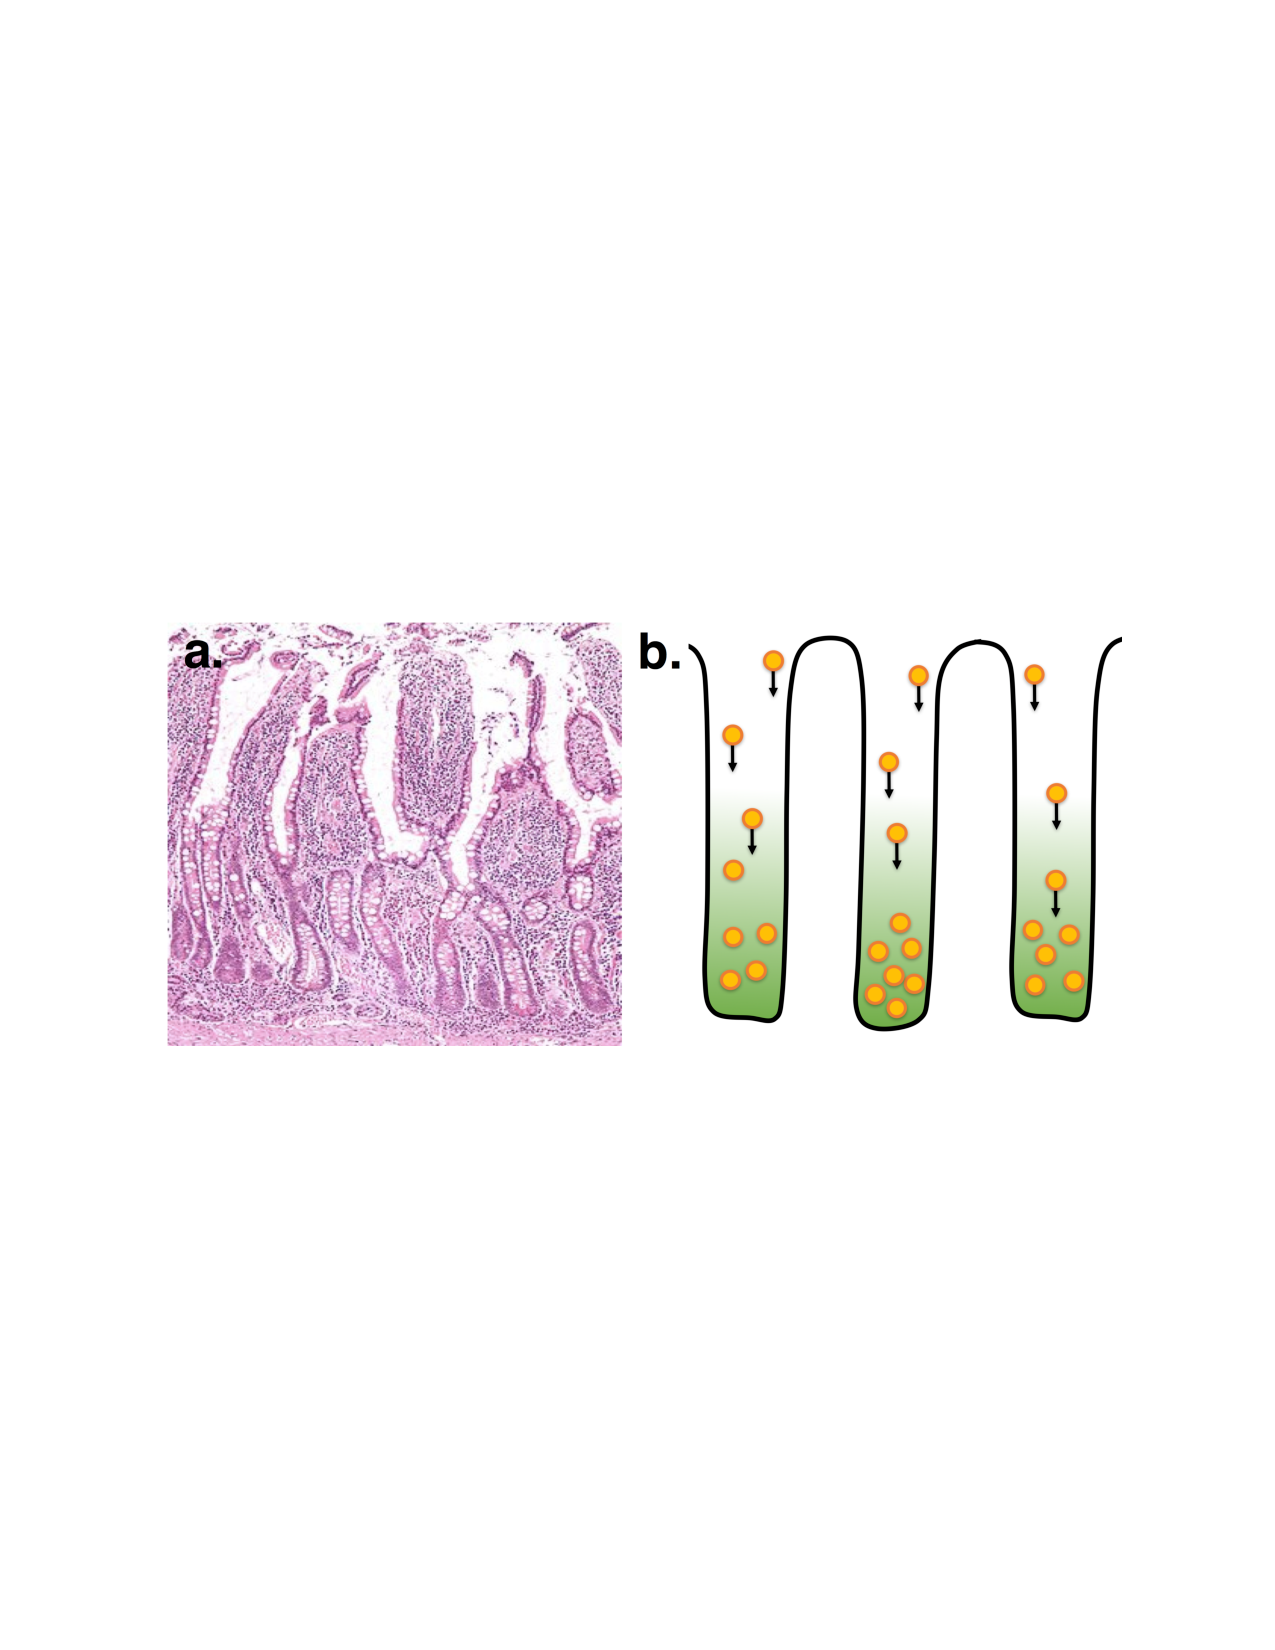
\includegraphics[width=2.2in]{figs/DeepPores.pdf}}
\vspace*{-11pt}
\caption{\label{fig:DeepPores} (a) Deep pores in intestinal villi, (b)
  targeted delivery of drug cargos in deep dead-end pores via
  osmophoresis.}
\end{wrapfigure}
The target areas are often located within deep pores such as intestine
(illustrated in Figure~\ref{fig:DeepPores}a), skin, lung, etc. In
practice, drug delivery in such locations relies on diffusion, which may
not be an effective mechanism, particularly for deep confined spaces. In
this regard, osmophoresis can be a potential mechanism for the effective
delivery of drug cargos (which are typically lipid vesicles) in deep
dead-end pores, as demonstrated in
Figure~\ref{fig:Microfluidic_dead-end} and Figure~\ref{fig:DeepPores}b. 

Chemicals are secreted and/or absorbed in such a way that a natural
gradient in the dead-end pore arises from the top to the deep end of the
pore, providing a suitable condition for osmophoresis toward the
dead-ends.  The PIs propose to investigate osmophoresis as a mechanism
to control the delivery of lipid vesicles in a corner flow (as in deep
dead-end pores) under a chemical gradient.  The PIs will focus on the
efficacy of vesicle transport to a target area in the pores using image
analysis and modeling.  As many lipidsomes exhibit different
permeabilities~\cite{fettiplace1980,olbrich2000}, control of the lipid
mixture ratio and vesicle size along with systematic experiments which
we gain from Aim I in \S\ref{subsec:aim1} will be utilized to design the
optimal cargo vesicles for targeted delivery. 

%%%%%%%%%%%%%%%%%%%%%%%%%%%%%%%%%%%%%%%%%%%%%%%%%%%%%%%%%%%%%%%%%%%%%%%%
\vspace*{-7pt}
\section{Management, Milestones and Budget}
\vspace*{-7pt}
%%  	
%\vspace*{-5pt}
\begin{wrapfigure}[15]{r}{3.1in}
\vspace*{-15pt}
\centerline{\includegraphics[width=3.1in]{figs/timeline.pdf}}
\vspace*{-8pt}
\caption{\label{fig:ScheduleMilestones} Schedule and milestones:
  Timeline for collaborative research activities.}
\end{wrapfigure}
%
The PIs will structure our work in steps to build synergies as we
proceed with the experiments and theoretical modeling. A schedule with
milestones of the main aspects of our proposed work is provided in
Figure~\ref{fig:ScheduleMilestones}. The main themes of this research
will be led by graduate students who will meet regularly with the PIs,
who will have responsibility for the budget and for preparing annual
reports. The data generated by the research, including experimental
results, numerical programs and mathematical modeling will be organized
and saved according to the Data Management Plan and will follow best
practices suggested by NSF. We will use the funding from this grant to
support graduate students during the academic year and the summer. The
budget includes funds for the graduate students to attend two
professional meetings a year (e.g. APS, ASME, SIAM and AIChE meetings).
The PIs will work with summer undergraduate students, as this engagement
with young researchers continues the PIs' outreach efforts. The budget
also includes a summer salary for SS as the PIs will work extensively
during the summer. The experimental work here is ideal for training
graduate and undergraduate students in experimental methods, image
processing and data analysis, basics of transport processes, etc.
Similarly, the mathematical modeling provides good projects for training
students and for encouraging comparison of experimental results with
quantitative models. In addition to the salary of two graduate students
and travel funds, we include funds for the various materials required to
perform the experiments: we need to purchase standard materials (e.g.
lipids, soft lithography materials, glassware, tubing, etc.), which will
be regular expenditures.
\todo[inline]{Reviewer 3 wanted to see a multiple PI leadership
arrangement (i.e., such as communication plan and conflict resolution,
andà) is missing.}


%%%%%%%%%%%%%%%%%%%%%%%%%%%%%%%%%%%%%%%%%%%%%%%%%%%%%%%%%%%%%%%%%%%%%%%%
\vspace*{-7pt}
\section{Educational Impacts and Outreach Program}
\label{sec:Educational_plans}
\vspace*{-7pt}

\todo[inline]{Reviewer 1 was critical of the educational impact}
\todo[inline]{Reviewer 3 was concerned with the assessment process for
outreach activities lack details. There is no indication of number of
high school students that will be involved. What type of learning
assessments will be measured?}

An important component of this proposal is the interdisciplinary
education and training of both undergraduate and graduate students. The
combination of microfluidics experiments, mathematical modeling, and
scientific computing in this project provides a compelling example of
the importance of interdisciplinary in biophysics. The proposed
experimental and numerical research will be integrated into an
educational effort directed toward students in Mechanical Engineering
and Applied Mathematics as well as an outreach effort aimed at
encouraging women and under-represented minority students such as
Pacific Islanders to the study of interdisciplinary biophysics. The
inherently interdisciplinary nature of the proposed experiment and
modeling is valuable for Mechanical Engineering students as the research
will provide exposure and training in aspects microfluidics engineering
such as soft lithography, microfabrication, and vesicle formation. In
this regard, SS has recently developed a lab session specifically
designed for the undergraduates (ME322) to learn and experience the
state-of-the-art microfluidics. ME322 have traditionally dealt with
classical fluid dynamics experiments but the newly designed
microfluidics lab is intended to expose the students to the latest
knowledge in the relevant field.  For Applied Mathematics students, the
proposed research program will enhance their training in mathematical
fluid modeling and computation. To evaluate the impact of and support
educational and training activities, the PIs and their groups will hold
regular group meetings, one-on-one tutorial sessions, and develop
web-based solutions (e.g., wiki-based and video tutorials, blogs,
live-streamed seminars).

The immediate educational impact of the proposed research will be on
undergraduate and graduate students involved in the research. On the
graduate-level education, PIs expect the projects to train and support
two PhD students for three years. PIs will foster close interaction
between the students and collaborators to enhance the interdisciplinary
learning environment. Research outcomes from the projects will be
broadly disseminated by publications in high-profile journals and
presentations in major national conferences such as APS and SIAM.
Numerical codes from these works will be made available to the public
and the community by posting on a dedicated website and published in
journal articles as supplementary.  The PIs expect to involve
undergraduate students in this project through their continuing and
active involvement in undergraduate advising and research mentoring: SS
has mentored native Hawaiian undergraduate students in effort to cherish
their educational background through Student Project Grants (SPG) and
Undergraduate Research Opportunities Program (UROP). SS has involved
undergraduate students in the UH microfabrication laboratory, and has
taught courses on fluid mechanics where he includes some of his recent
research as one of the topics. YNY has mentored undergraduate students
as a co-Investigator in CSUMS: Research and Education in Computational
Mathematics for undergraduates in the Mathematical Sciences at NJIT
(funded by NSF) and the lecturer for Capstone Applied Mathematics Lab at
NJIT (also funded by NSF).  In addition, both PIs will continue to make
outreach efforts to actively recruit indigenous Pacific Islanders,
female and under-represented minority high school students through the
PIs' participation in (a) the Summer Scholar Program and Education-USA
Academy Program at UH (SS), and (b) the outreach program of TECHS-NJ,
Teacher Education Collaboration for High-Need Schools-NJ (YNY).

%%%%%%%%%%%%%%%%%%%%%%%%%%%%%%%%%%%%%%%%%%%%%%%%%%%%%%%%%%%%%%%%%%%%%%%%
\vspace*{-7pt}
\section{Results from Prior Relevant NSF Support}
\vspace*{-7pt}

\noindent
PI Shin has no prior relevant research support from NSF.

\noindent
PI Young: {\it NSF-DMS-1222550, Mathematical and experimental study of
lipid bilayer shape and dynamics mediated by surfactants and proteins},
\$212,603, 9/15/2012 - 08/31/2016, PI.  The focus of this grant is
modeling the interaction between a pure lipid bilayer membrane with
surfactant, cholesterol and protein.  Hence, there is no overlap between
these grants and the current proposal.

\noindent
{\it Intellectual merit:} YNY and collaborators have studied (1)
asymmetry of lipid bilayer due to its interaction with proteins and
surfactants, (2) the electrohydrodynamics of a LBM under an electric
field, and (3) the coupling between LBM dynamics and a transmembrane
protein, such as a mechanosensitive channel. 

\noindent
{\it Broader impacts:} 
One PhD student (Szu-Pei Fu) is funded to work with YNY, and work has
resulted in seven papers~\cite{Nganguia2013_PoF, Nganguia2013_PRE,
Young2014_JFM, Young2015_PoF, Nganguia2015_CiCP, Pak2015, Fu2015_PRE}.
YNY has been actively involved with promotion of minority students at
NJIT.  One of his two PhD students (Herve Nganguia) is African. YNY has
taught a broad spectrum of courses in fluid mechanics, applied math
modeling, and complex flows.


\newpage

%\bibliographystyle{plain}
\bibliographystyle{unsrt}

\bibliography{bibliography_SSd,AM2015,bibQuaife}

\end{document}
